\documentclass[a4paper,12pt]{book}
\usepackage[utf8]{inputenc}
\title{}
\author{Rachel Morris}
\date{\today}

\usepackage{rachwidgets}
\usepackage{fancyhdr}
\usepackage{lastpage}
\usepackage{dirtree}
\usepackage{boxedminipage}

\setcounter{chapter}{3}
\setcounter{section}{4}
\newcommand{\laChapter}{3.5 Logic Circuits\ }
\newcounter{question}

\newcommand{\laClass}{CS 210\ }
\newcommand{\laSemester}{Fall 2017\ }

\pagestyle{fancy}
\fancyhf{}
\lhead{\laClass \laSemester}
\chead{}
\rhead{Ch \laChapter}
\rfoot{\thepage\ of \pageref{LastPage}}
\lfoot{\scriptsize Compiled by Rachel Morris, last updated \today}

\renewcommand{\headrulewidth}{2pt}
\renewcommand{\footrulewidth}{1pt}

\begin{document}

    %\toggletrue{answerkey}
    \togglefalse{answerkey}

    %------------------------------------------------------------------%
    %- Exercise Begin -------------------------------------------------%
    %------------------------------------------------------------------%

    \section{Logic Circuits}

	\subsection{Logic Circuits}
	
	\begin{intro}{\ }
		We are going to be using logic gates as one way to represent our
		Boolean Algebra expressions graphically. The gates that we will be using are:
		
		\begin{center}
			\begin{tabular}{c c c}
				AND $\cdot$ & OR $+$ & NOT $'$ \\
				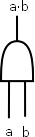
\includegraphics[height=4cm]{images/3-5-andgate.png} &
				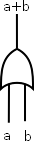
\includegraphics[height=4cm]{images/3-5-orgate.png} &
				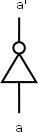
\includegraphics[height=4cm]{images/3-5-notgate.png} 
				\\ \\
				\begin{tabular}{ c c | c }
					$a$ & $b$ & $a \cdot b$ \\ \hline
					0 & 0 & 0 \\
					0 & 1 & 0 \\
					1 & 0 & 0 \\
					1 & 1 & 1
				\end{tabular}
				&
				
				\begin{tabular}{ c c | c }
					$a$ & $b$ & $a + b$ \\ \hline
					0 & 0 & 0 \\
					0 & 1 & 1 \\
					1 & 0 & 1 \\
					1 & 1 & 1
				\end{tabular}
				&
				
				\begin{tabular}{ c | c }
					$a$ & $a'$ \\ \hline
					0 & 1 \\
					1 & 0 
				\end{tabular}
			\end{tabular}
			
		\end{center}
		
			~\\
			Additionally, we can connect gates together in order to build an expression. 
			For example:
			
		\begin{center}
			\begin{tabular}{c c c}
				$(a+b)'$ &
				$ ab + a'b $ &
				$(a+b) \cdot (b' + c)$
				\\
				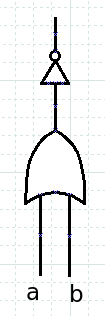
\includegraphics[height=6cm]{images/3-5-gate1.png} &
				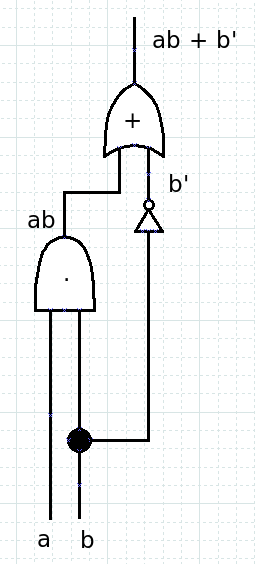
\includegraphics[height=6cm]{images/3-5-gate2.png} &
				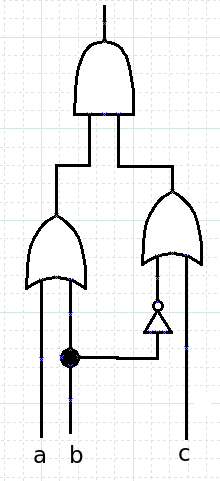
\includegraphics[height=6cm]{images/3-5-gate3.png} 
			\end{tabular}
		\end{center}
			
	\end{intro}
		
		\newpage
		
        % - QUESTION --------------------------------------------------%
        \stepcounter{question}
        \begin{questionNOGRADE}{\thequestion}
			
			Write out the Boolean expression that describes each diagram:
	
			
        \end{questionNOGRADE}
        
        \hrulefill
		
        % - QUESTION --------------------------------------------------%
        \stepcounter{question}
        \begin{questionNOGRADE}{\thequestion}
			
			Draw a circuit diagram for the following Boolean expressions:
			
			\begin{tabular}{p{4cm} p{4cm} p{4cm}}
				a. $a + b'$ &
				b. $a' \cdot b'$ &
				c. $a + (b \cdot c)$
			\end{tabular}

			
        \end{questionNOGRADE}
        
        
        

\end{document}








